\documentclass{standalone}
\usepackage{tikz}
\usetikzlibrary{patterns, positioning}
\usepackage[sfdefault]{ClearSans} %% option 'sfdefault' activates Clear Sans as the default text font
\usepackage[T1]{fontenc}

\begin{document}
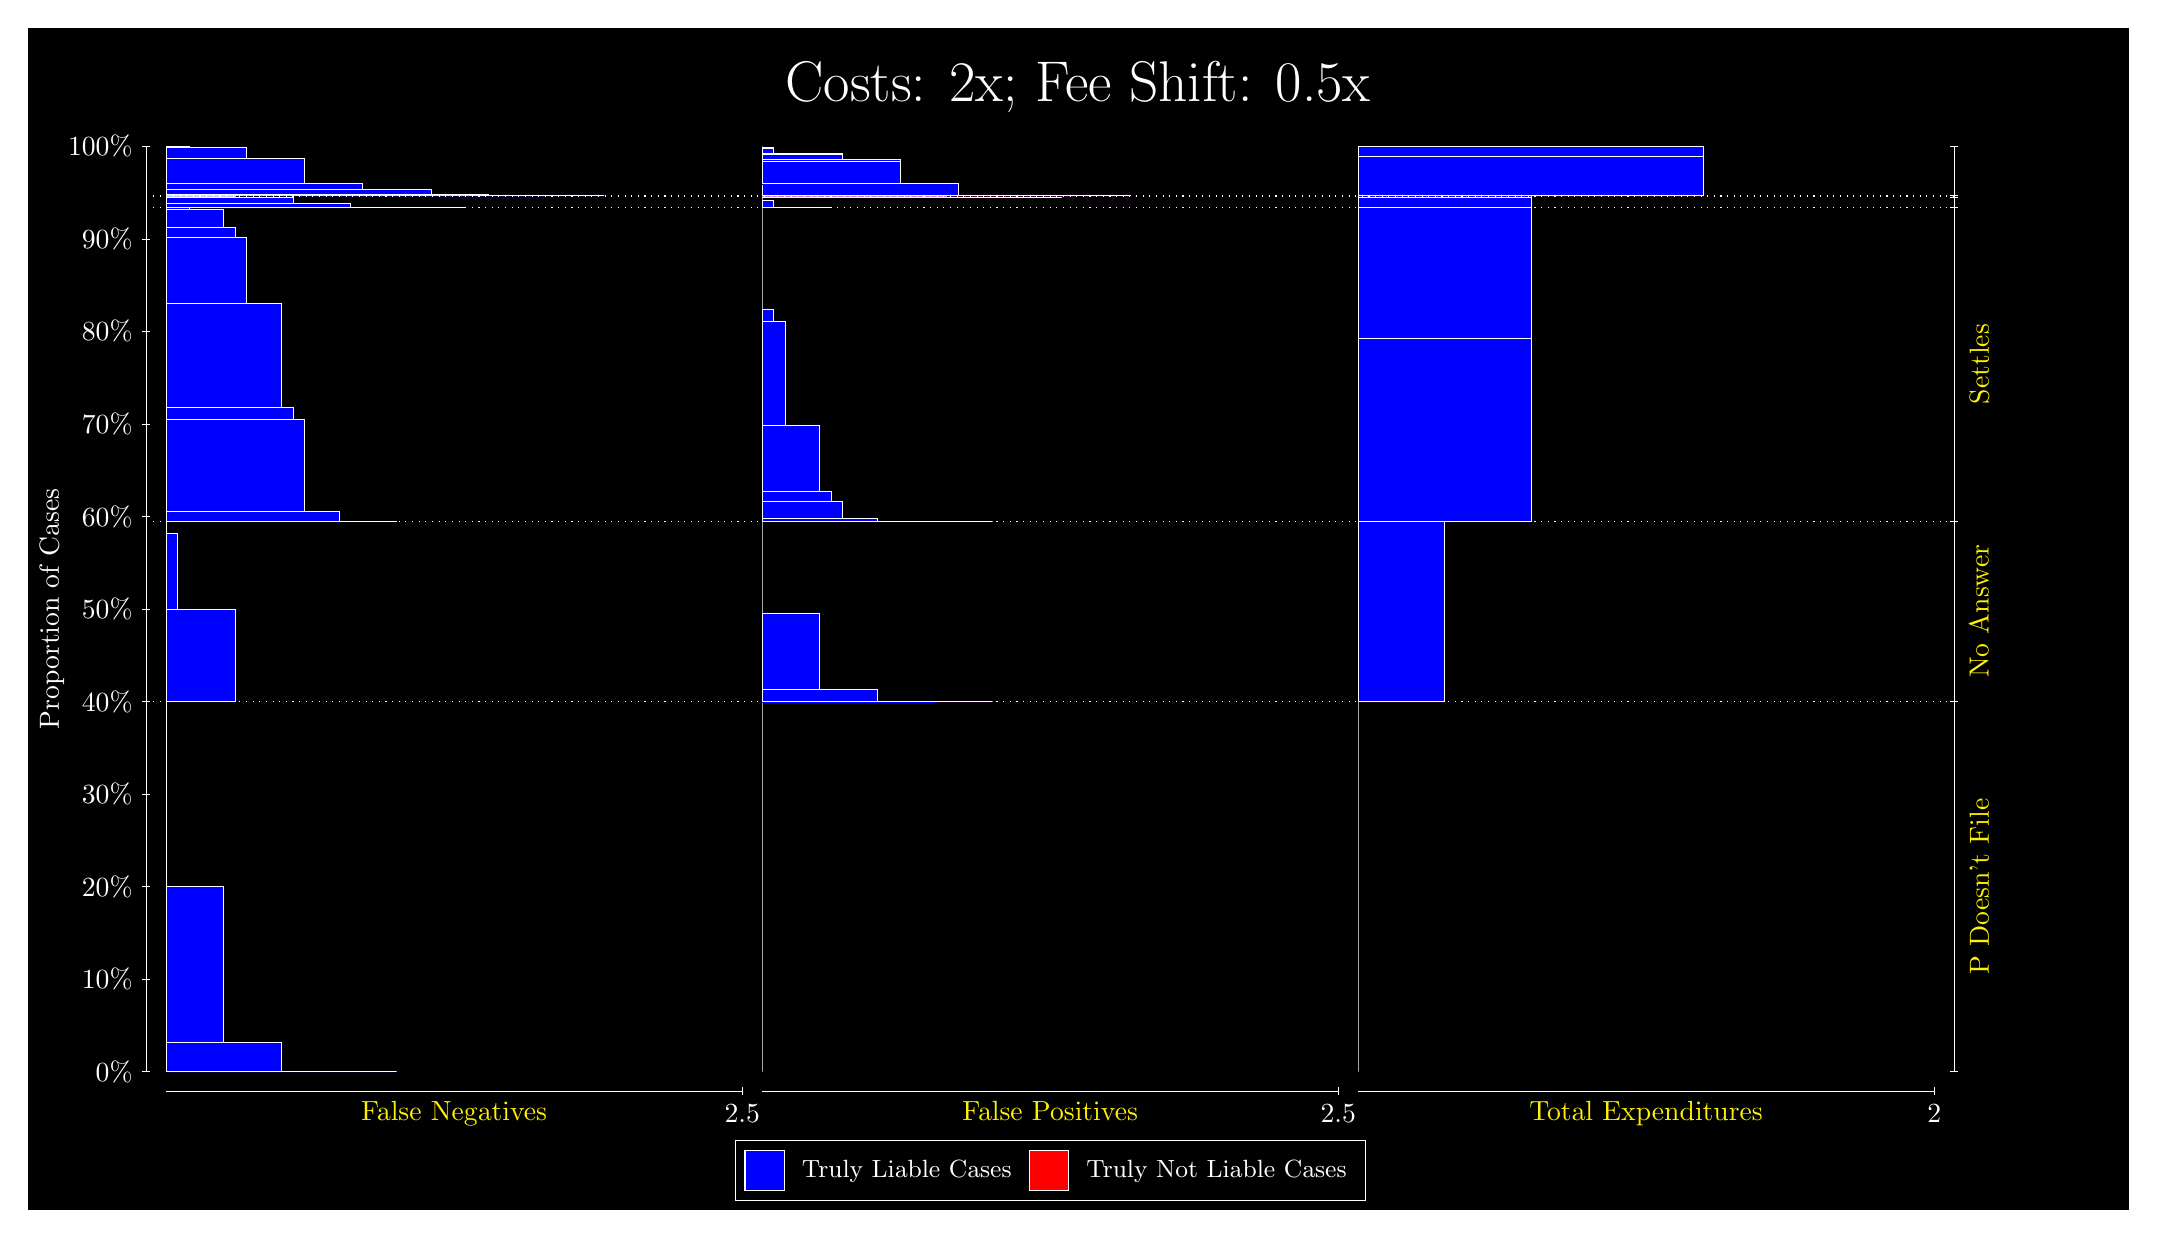
\begin{tikzpicture}
\draw[fill=black] (0,0) rectangle (26.667,15);
\draw[text=white] (0,13.5) rectangle (26.667,15) node[midway] {\huge Costs: 2x; Fee Shift: 0.5x};
\draw[white, very thin] (1.5,1.75) -- (1.5,13.5);
\node[rotate=90, text=white, anchor=center] at (0.3, 7.625) {Proportion of Cases};
\draw[white, very thin] (1.45,1.75) -- (1.55,1.75);
\node[text=white, anchor=east] at (1.45, 1.75) {0\%};
\draw[white, very thin] (1.45,2.925) -- (1.55,2.925);
\node[text=white, anchor=east] at (1.45, 2.925) {10\%};
\draw[white, very thin] (1.45,4.1) -- (1.55,4.1);
\node[text=white, anchor=east] at (1.45, 4.1) {20\%};
\draw[white, very thin] (1.45,5.275) -- (1.55,5.275);
\node[text=white, anchor=east] at (1.45, 5.275) {30\%};
\draw[white, very thin] (1.45,6.45) -- (1.55,6.45);
\node[text=white, anchor=east] at (1.45, 6.45) {40\%};
\draw[white, very thin] (1.45,7.625) -- (1.55,7.625);
\node[text=white, anchor=east] at (1.45, 7.625) {50\%};
\draw[white, very thin] (1.45,8.8) -- (1.55,8.8);
\node[text=white, anchor=east] at (1.45, 8.8) {60\%};
\draw[white, very thin] (1.45,9.975) -- (1.55,9.975);
\node[text=white, anchor=east] at (1.45, 9.975) {70\%};
\draw[white, very thin] (1.45,11.15) -- (1.55,11.15);
\node[text=white, anchor=east] at (1.45, 11.15) {80\%};
\draw[white, very thin] (1.45,12.325) -- (1.55,12.325);
\node[text=white, anchor=east] at (1.45, 12.325) {90\%};
\draw[white, very thin] (1.45,13.5) -- (1.55,13.5);
\node[text=white, anchor=east] at (1.45, 13.5) {100\%};

\draw[white, very thin] (24.457,1.75) -- (24.457,13.5);
\draw[white, very thin] (24.407,1.75) -- (24.507,1.75);
\node[anchor=west] at (24.407, 1.75) {};
\draw[white, very thin] (24.407,6.4489) -- (24.507,6.4489);
\node[anchor=west] at (24.407, 6.4489) {};
\draw[white, very thin] (24.407,8.7409) -- (24.507,8.7409);
\node[anchor=west] at (24.407, 8.7409) {};
\draw[white, very thin] (24.407,12.727) -- (24.507,12.727);
\node[anchor=west] at (24.407, 12.727) {};
\draw[white, very thin] (24.407,12.859) -- (24.507,12.859);
\node[anchor=west] at (24.407, 12.859) {};
\draw[white, very thin] (24.407,12.874) -- (24.507,12.874);
\node[anchor=west] at (24.407, 12.874) {};
\draw[white, very thin] (24.407,13.5) -- (24.507,13.5);
\node[anchor=west] at (24.407, 13.5) {};

\draw[white, very thin, fill=blue] (1.75,1.75) rectangle (4.6775,1.75);
\draw[white, very thin, fill=blue] (1.75,1.75) rectangle (3.9457,1.7532);
\draw[white, very thin, fill=blue] (1.75,1.7532) rectangle (3.2138,2.126);
\draw[white, very thin, fill=blue] (1.75,2.126) rectangle (2.4819,4.1027);
\draw[white, very thin, fill=red] (1.75,4.1027) rectangle (1.75,4.1027);
\draw[white, very thin, fill=blue] (1.75,4.1027) rectangle (1.75,6.4489);
\draw[white, very thin, fill=blue] (1.75,6.4489) rectangle (2.6283,7.6173);
\draw[white, very thin, fill=blue] (1.75,7.6173) rectangle (1.8964,8.5872);
\draw[white, very thin, fill=red] (1.75,8.5872) rectangle (1.75,8.5872);
\draw[white, very thin, fill=blue] (1.75,8.5872) rectangle (1.75,8.7409);
\draw[white, very thin, fill=blue] (1.75,8.7409) rectangle (4.6775,8.7414);
\draw[white, very thin, fill=blue] (1.75,8.7414) rectangle (4.092,8.7433);
\draw[white, very thin, fill=blue] (1.75,8.7433) rectangle (3.9457,8.8611);
\draw[white, very thin, fill=blue] (1.75,8.8611) rectangle (3.5065,10.032);
\draw[white, very thin, fill=blue] (1.75,10.032) rectangle (3.3602,10.188);
\draw[white, very thin, fill=blue] (1.75,10.188) rectangle (3.2138,11.512);
\draw[white, very thin, fill=blue] (1.75,11.512) rectangle (2.7746,12.344);
\draw[white, very thin, fill=blue] (1.75,12.344) rectangle (2.6283,12.471);
\draw[white, very thin, fill=blue] (1.75,12.471) rectangle (2.4819,12.697);
\draw[white, very thin, fill=blue] (1.75,12.697) rectangle (2.0428,12.727);
\draw[white, very thin, fill=blue] (1.75,12.727) rectangle (1.8964,12.727);
\draw[white, very thin, fill=red] (1.75,12.727) rectangle (1.75,12.727);
\draw[white, very thin, fill=blue] (1.75,12.727) rectangle (1.75,12.727);
\draw[white, very thin, fill=blue] (1.75,12.727) rectangle (5.5558,12.727);
\draw[white, very thin, fill=blue] (1.75,12.727) rectangle (4.8239,12.727);
\draw[white, very thin, fill=blue] (1.75,12.727) rectangle (4.092,12.777);
\draw[white, very thin, fill=blue] (1.75,12.777) rectangle (3.3602,12.858);
\draw[white, very thin, fill=blue] (1.75,12.858) rectangle (2.6283,12.859);
\draw[white, very thin, fill=red] (1.75,12.859) rectangle (1.75,12.859);
\draw[white, very thin, fill=blue] (1.75,12.859) rectangle (2.6283,12.864);
\draw[white, very thin, fill=blue] (1.75,12.864) rectangle (1.8964,12.873);
\draw[white, very thin, fill=red] (1.75,12.873) rectangle (1.75,12.873);
\draw[white, very thin, fill=blue] (1.75,12.873) rectangle (1.75,12.874);
\draw[white, very thin, fill=blue] (1.75,12.874) rectangle (7.3123,12.874);
\draw[white, very thin, fill=blue] (1.75,12.874) rectangle (6.5805,12.874);
\draw[white, very thin, fill=blue] (1.75,12.874) rectangle (5.8486,12.886);
\draw[white, very thin, fill=blue] (1.75,12.886) rectangle (5.7022,12.886);
\draw[white, very thin, fill=blue] (1.75,12.886) rectangle (5.1167,12.956);
\draw[white, very thin, fill=blue] (1.75,12.956) rectangle (4.9703,12.956);
\draw[white, very thin, fill=blue] (1.75,12.956) rectangle (4.3848,12.958);
\draw[white, very thin, fill=blue] (1.75,12.958) rectangle (4.2384,13.034);
\draw[white, very thin, fill=blue] (1.75,13.034) rectangle (3.6529,13.034);
\draw[white, very thin, fill=blue] (1.75,13.034) rectangle (3.5065,13.347);
\draw[white, very thin, fill=blue] (1.75,13.347) rectangle (2.7746,13.492);
\draw[white, very thin, fill=blue] (1.75,13.492) rectangle (2.0428,13.5);
\draw[white, very thin, fill=red] (1.75,13.5) rectangle (1.75,13.5);
\draw[white, very thin, fill=blue] (1.75,13.5) rectangle (1.75,13.5);
\draw[white, very thin, fill=red] (9.3189,1.75) rectangle (9.3189,1.75);
\draw[white, very thin, fill=blue] (9.3189,1.75) rectangle (9.3189,6.4489);
\draw[white, very thin, fill=red] (9.3189,6.4489) rectangle (12.246,6.4489);
\draw[white, very thin, fill=blue] (9.3189,6.4489) rectangle (12.246,6.4489);
\draw[white, very thin, fill=blue] (9.3189,6.4489) rectangle (11.515,6.4492);
\draw[white, very thin, fill=blue] (9.3189,6.4492) rectangle (10.783,6.6027);
\draw[white, very thin, fill=blue] (9.3189,6.6027) rectangle (10.051,7.5725);
\draw[white, very thin, fill=blue] (9.3189,7.5725) rectangle (9.3189,8.7409);
\draw[white, very thin, fill=red] (9.3189,8.7409) rectangle (12.246,8.7409);
\draw[white, very thin, fill=blue] (9.3189,8.7409) rectangle (12.246,8.7409);
\draw[white, very thin, fill=red] (9.3189,8.7409) rectangle (11.661,8.7409);
\draw[white, very thin, fill=blue] (9.3189,8.7409) rectangle (11.661,8.7409);
\draw[white, very thin, fill=blue] (9.3189,8.7409) rectangle (11.515,8.7409);
\draw[white, very thin, fill=red] (9.3189,8.7409) rectangle (11.075,8.7409);
\draw[white, very thin, fill=blue] (9.3189,8.7409) rectangle (11.075,8.7414);
\draw[white, very thin, fill=blue] (9.3189,8.7414) rectangle (10.929,8.7416);
\draw[white, very thin, fill=blue] (9.3189,8.7416) rectangle (10.783,8.7712);
\draw[white, very thin, fill=blue] (9.3189,8.7712) rectangle (10.344,8.9974);
\draw[white, very thin, fill=blue] (9.3189,8.9974) rectangle (10.197,9.1246);
\draw[white, very thin, fill=blue] (9.3189,9.1246) rectangle (10.051,9.956);
\draw[white, very thin, fill=blue] (9.3189,9.956) rectangle (9.6116,11.28);
\draw[white, very thin, fill=blue] (9.3189,11.28) rectangle (9.4652,11.436);
\draw[white, very thin, fill=blue] (9.3189,11.436) rectangle (9.3189,12.727);
\draw[white, very thin, fill=red] (9.3189,12.727) rectangle (10.197,12.727);
\draw[white, very thin, fill=blue] (9.3189,12.727) rectangle (10.197,12.729);
\draw[white, very thin, fill=blue] (9.3189,12.729) rectangle (9.4652,12.81);
\draw[white, very thin, fill=blue] (9.3189,12.81) rectangle (9.3189,12.859);
\draw[white, very thin, fill=red] (9.3189,12.859) rectangle (13.125,12.859);
\draw[white, very thin, fill=blue] (9.3189,12.859) rectangle (13.125,12.859);
\draw[white, very thin, fill=blue] (9.3189,12.859) rectangle (12.393,12.859);
\draw[white, very thin, fill=blue] (9.3189,12.859) rectangle (11.661,12.86);
\draw[white, very thin, fill=blue] (9.3189,12.86) rectangle (10.929,12.869);
\draw[white, very thin, fill=blue] (9.3189,12.869) rectangle (10.197,12.874);
\draw[white, very thin, fill=red] (9.3189,12.874) rectangle (14.003,12.874);
\draw[white, very thin, fill=blue] (9.3189,12.874) rectangle (14.003,12.874);
\draw[white, very thin, fill=red] (9.3189,12.874) rectangle (13.271,12.874);
\draw[white, very thin, fill=blue] (9.3189,12.874) rectangle (13.271,12.874);
\draw[white, very thin, fill=red] (9.3189,12.874) rectangle (12.539,12.874);
\draw[white, very thin, fill=blue] (9.3189,12.874) rectangle (12.539,12.882);
\draw[white, very thin, fill=blue] (9.3189,12.882) rectangle (11.807,13.026);
\draw[white, very thin, fill=red] (9.3189,13.026) rectangle (11.807,13.026);
\draw[white, very thin, fill=blue] (9.3189,13.026) rectangle (11.807,13.027);
\draw[white, very thin, fill=blue] (9.3189,13.027) rectangle (11.075,13.307);
\draw[white, very thin, fill=blue] (9.3189,13.307) rectangle (11.075,13.34);
\draw[white, very thin, fill=red] (9.3189,13.34) rectangle (10.929,13.34);
\draw[white, very thin, fill=blue] (9.3189,13.34) rectangle (10.929,13.34);
\draw[white, very thin, fill=blue] (9.3189,13.34) rectangle (10.344,13.403);
\draw[white, very thin, fill=blue] (9.3189,13.403) rectangle (10.344,13.416);
\draw[white, very thin, fill=blue] (9.3189,13.416) rectangle (10.197,13.417);
\draw[white, very thin, fill=red] (9.3189,13.417) rectangle (10.197,13.417);
\draw[white, very thin, fill=blue] (9.3189,13.417) rectangle (10.197,13.418);
\draw[white, very thin, fill=blue] (9.3189,13.418) rectangle (9.6116,13.418);
\draw[white, very thin, fill=blue] (9.3189,13.418) rectangle (9.6116,13.418);
\draw[white, very thin, fill=blue] (9.3189,13.418) rectangle (9.4652,13.472);
\draw[white, very thin, fill=blue] (9.3189,13.472) rectangle (9.4652,13.487);
\draw[white, very thin, fill=blue] (9.3189,13.487) rectangle (9.3189,13.5);
\draw[white, very thin, fill=red] (16.888,1.75) rectangle (16.888,1.75);
\draw[white, very thin, fill=blue] (16.888,1.75) rectangle (16.888,6.4489);
\draw[white, very thin, fill=red] (16.888,6.4489) rectangle (17.986,6.4489);
\draw[white, very thin, fill=blue] (16.888,6.4489) rectangle (17.986,8.7409);
\draw[white, very thin, fill=red] (16.888,8.7409) rectangle (19.083,8.7409);
\draw[white, very thin, fill=blue] (16.888,8.7409) rectangle (19.083,11.058);
\draw[white, very thin, fill=red] (16.888,11.058) rectangle (19.083,11.058);
\draw[white, very thin, fill=blue] (16.888,11.058) rectangle (19.083,12.727);
\draw[white, very thin, fill=red] (16.888,12.727) rectangle (19.083,12.727);
\draw[white, very thin, fill=blue] (16.888,12.727) rectangle (19.083,12.859);
\draw[white, very thin, fill=red] (16.888,12.859) rectangle (19.083,12.859);
\draw[white, very thin, fill=blue] (16.888,12.859) rectangle (19.083,12.874);
\draw[white, very thin, fill=red] (16.888,12.874) rectangle (21.279,12.874);
\draw[white, very thin, fill=blue] (16.888,12.874) rectangle (21.279,13.37);
\draw[white, very thin, fill=red] (16.888,13.37) rectangle (21.279,13.37);
\draw[white, very thin, fill=blue] (16.888,13.37) rectangle (21.279,13.5);
\draw[white, dotted] (1.5,6.4489) -- (24.457,6.4489);
\draw[white, dotted] (1.5,8.7409) -- (24.457,8.7409);
\draw[white, dotted] (1.5,12.727) -- (24.457,12.727);
\draw[white, dotted] (1.5,12.859) -- (24.457,12.859);
\draw[white, dotted] (1.5,12.874) -- (24.457,12.874);
\draw[white, very thin] (1.75,1.5) -- (9.0689,1.5);
\node[text=yellow, anchor=north] at (5.4094, 1.5) {False Negatives};
\draw[white, very thin] (9.0689,1.45) -- (9.0689,1.55);
\node[text=white, anchor=north] at (9.0689, 1.45) {2.5};

\draw[white, very thin] (9.3189,1.5) -- (16.638,1.5);
\node[text=yellow, anchor=north] at (12.978, 1.5) {False Positives};
\draw[white, very thin] (16.638,1.45) -- (16.638,1.55);
\node[text=white, anchor=north] at (16.638, 1.45) {2.5};

\draw[white, very thin] (16.888,1.5) -- (24.207,1.5);
\node[text=yellow, anchor=north] at (20.547, 1.5) {Total Expenditures};
\draw[white, very thin] (24.207,1.45) -- (24.207,1.55);
\node[text=white, anchor=north] at (24.207, 1.45) {2};

\node[text=yellow, centered, rotate=90] at (24.777, 4.0995) {P Doesn't File};
\node[text=yellow, centered, rotate=90] at (24.777, 7.5949) {No Answer};
\node[text=yellow, centered, rotate=90] at (24.777, 10.734) {Settles};




\draw (12.978300999999998,1.5) node[draw=none] (baseCoordinate) {};
\begin{scope}[align=center]
        \matrix[scale=0.5, draw=white, below=0.5cm of baseCoordinate, nodes={draw}, column sep=0.1cm]{
            \node[rectangle, draw, minimum width=0.5cm, minimum height=0.5cm, fill=blue] {}; &
            \node[draw=none, font=\small, text=white] (B) {Truly Liable Cases}; &
            \node[rectangle, draw, minimum width=0.5cm, minimum height=0.5cm, fill=red] {}; &
            \node[draw=none, font=\small, text=white] (B) {Truly Not Liable Cases}; \\
            };
\end{scope}

\end{tikzpicture}
\end{document}